\section{Algunas propiedades de $\Sigma_{x}$}

Antes de continuar, 
fijada una dimensión $n \geq 2$ y una 
señal $x \in \IR^{n}$,
establezcamos algunas propiedades de la función
$\Sigma_{x}: [0, \infty[ \longrightarrow$ definida como

\begin{equation}
\label{eq: estudiando espectro}
\Sigma_{x}(\omega) := \sigma_{n}(x, \omega),
\end{equation}
donde los coeficientes $\sigma_{n}(x, \omega)$
son como se definieron en 
\eqref{eq: def sigmas}, 
pues, al ser la función que a cada
frecuencia positiva le asigna el coseno del 
ángulo que $x$ forma con el espacio monofrecuencial
$P_{n, \omega}$, parece en principio ser una buena candidata
a espectro de $x$. Tales propiedades nos ayudarán a afinar tal
definición, y dar así una definición del espectro
de una señal basado en espacios monofrecuenciales.


El primer resultado de esta sección establece
la periodicidad del espectro, hecho que
nos permitirá
acotar considerablemente el dominio de frecuencias
de la función $\Sigma_{x}$.

\subsection{Periodicidad}
\begin{prop}
\label{prop: periodicidad espectro}
\textbf{(Periodicidad de la función \eqref{eq: estudiando espectro})}
Sean $n \geq 2$, $x \in \IR^{n}$.
Sea $\Sigma_{x}$ la función definida como en 
\eqref{eq: estudiando espectro}. La función 
$\Sigma_{x}$ $n-$periódica, es decir, 
para cualquier frecuencia
$0 \leq \omega \leq n$
y toda $K \in \IZ$, se tiene que 
\[
\sigma_{n}(x, \omega) = \sigma_{n}(x, \omega + Kn).
\]
\end{prop}
\noindent
\textbf{Demostración.}
Sólo observe que 
\begin{align*}
\tilde{c}_{n, \omega + Kn} = & \left( cos \left( 2 \pi
\left( \omega + Kn \right) \frac{m}{n} \right) \right)_{m=0}^{n-1} \\
= & \left( cos \left( 
2 \pi \omega \frac{m}{n} + 2 \pi K m
\right) \right)_{m=0}^{n-1} \\
= & \left( cos \left( 
2 \pi \omega \frac{m}{n}
\right) \right)_{m=0}^{n-1} = \tilde{c}_{n, \omega}
\end{align*}
y, similarmente, que 
\[
\tilde{s}_{n, \omega + Kn} = \tilde{s}_{n, \omega},
\]
luego, por definición de los espacios monofrecuenciales
(c.f. ecuación \ref{eq: espacio Pnw}),
\begin{align*}
P_{n, \omega + Kn} =
& span(\tilde{c}_{n, \omega + Kn}, \tilde{s}_{n, \omega + Kn}) \\
= & span(\tilde{c}_{n, \omega }, \tilde{s}_{n, \omega }) = P_{n, \omega};
\end{align*}
de esto se concluye, usando la definición
\ref{def: final de sigmas},
que 
\[
\sigma_{n}(x, \omega) = 
cos (\measuredangle(x, P_{n, \omega}))
= cos (\measuredangle(x, P_{n, \omega + Kn})) = 
\sigma_{n}(x, \omega + Kn).
\]
\QEDB
\vspace{0.2cm}

\begin{figure}[H]
	\sidecaption{
	Según la periodicidad establecida en la proposición 
	\ref{prop: periodicidad espectro}, basta calcular los
	coeficientes espectrales
	$\sigma_{n}(x, \omega)$ para frecuencias
	$0 \leq \omega \leq n$.
	\label{fig: periodicidad espectro}
	}
	\centering
	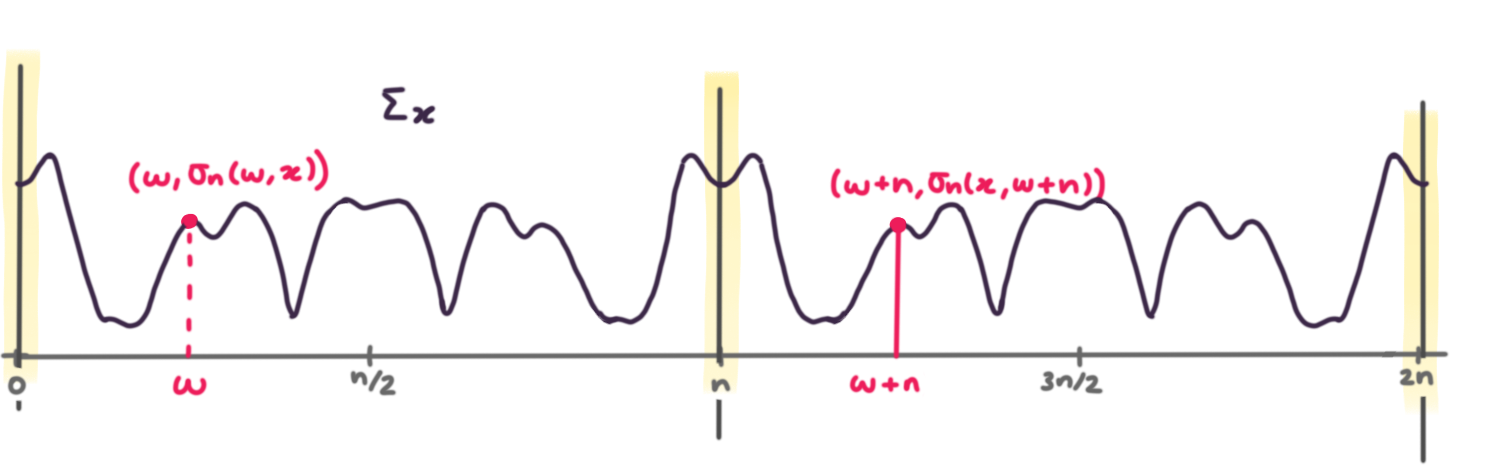
\includegraphics[scale = 0.9]{periodicidad_espectro} 
\end{figure}	


\subsection{Simetría}
\begin{prop}
\label{ref: simetria espectro}
\textbf{(Simetría de la función
\eqref{eq: estudiando espectro})}
Sean
$n \geq 2$,
$x \in \IR^{n}$. Para toda $0 \leq \omega \leq \frac{n}{2}$,
\[
\Sigma_{x}(\omega) = \Sigma_{x}(n-\omega).
\]
\end{prop}
\noindent
\textbf{Demostración.}
Debemos demostrar que se tiene la igualdad 
\[
\sigma_{n}(x, \omega) = 
\sigma_{n}(x, n-\omega ).
\]
En efecto, 
\begin{align*}
\tilde{c}_{n, \omega + n} = & \left( cos \left( 2 \pi
\left( n- \omega \right) \frac{m}{n} \right) \right)_{m=0}^{n-1} \\
= & \left( cos \left( 
2 \pi n \frac{m}{n} - 2 \pi \omega
\frac{m}{n}
\right) \right)_{m=0}^{n-1} \\
= & \left( cos \left( 
2 \pi m - 2 \pi \omega \frac{m}{n} 
\right) \right)_{m=0}^{n-1} \\
= & \left( cos \left( 2 \pi \omega \frac{m}{n} \right) \right)_{m=0}^{n-1}
= \tilde{c}_{n, \omega}
\end{align*}
y, similarmente,
\[
\tilde{s}_{n, \omega + Kn} = -\tilde{s}_{n, \omega};
\]
de esto, como en la demostración de la proposición
\ref{prop: periodicidad espectro}, se concluye la igualdad
entre los espacios $P_{n, \omega}$ y $P_{n, n-\omega}$, y de esto
la igualdad deseada.
\QEDB
\vspace{0.2cm}

\begin{figure}[H]
	\sidecaption{
	Podemos así afinar la afirmación hecha en la figura 
	\ref{fig: periodicidad espectro} y concluir que basta
	calcular los coeficientes
	$\sigma_{n}(x, \omega)$ para $0 \leq \omega \leq \frac{n}{2}$,
	pues los demás pueden deducirse a partir de reflexiones y traslaciones.
	\label{fig: simetria espectro}
	}
	\centering
	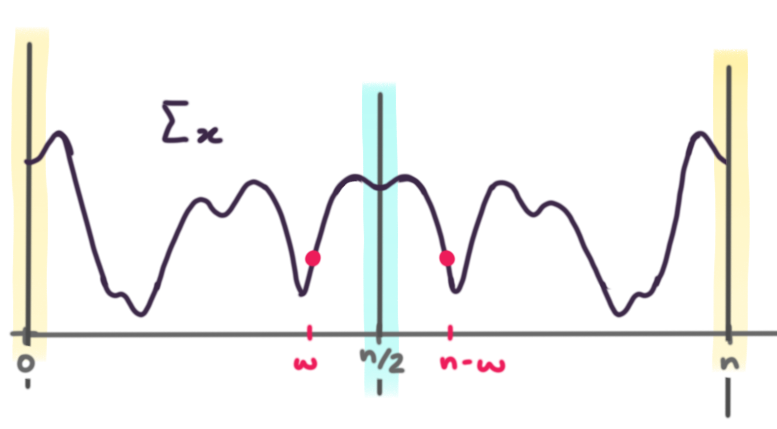
\includegraphics[scale = 1.4]{simetria_espectro} 
\end{figure}	
 

\begin{nota}
\label{nota: muestreo dom frecuencia}
Según estas propiedades de periodicidad y simetría,
podemos limitarnos a evaluar la función
$\Sigma_{x}$ sólo en frecuencias
contenidas en el intervalo $[0, n/2]$, pues los valores
del espectro para otros valores pueden deducirse por periodicidad
y simetría. \\

\TODO{tal vez debería mover esto.}
Ahora bien, para poder escribir programas
para calcular una tal función $\Sigma_{x}$,
se debe de usar como dominio de esta
un conjunto discreto de puntos.
Para los espectros que calcularemos de ahora en 
adelante, adoptamos la convención de 
usar usar como dominio 
de la función
$\Sigma_{x}$ de una señal $x \in \IR^{n}$
al conjunto
\begin{equation}
\label{eq: malla frecuencias}
\left\{ \frac{a}{100} : \hspace{0.2cm}
0 \leq a \leq 
\left\lfloor\frac{100n}{2}\right\rfloor,
\right\}
\end{equation}

\noindent
es decir, se toman $100$ muestras por
cada unidad del intervalo 
$\left[ 0, \frac{n}{2}\right]$
\end{nota}

\subsection{Continuidad}

Fijada una $n \geq 2$ y una $x \in \IR^{n}$,
vamos a analizar la continuidad de la función
$\Sigma_{x}$ como se definió 
en \eqref{eq: estudiando espectro}.
Por la periodicidad y simetría establecidas
en las proposiciones 
\ref{prop: periodicidad espectro}
y \ref{ref: simetria espectro}, basta
analizar la continuidad de $\Sigma_{x}$ sólo en el
intervalo cerrado $[0, n/2]$. Establecer la continuidad
de $\Sigma_{x}$ en el interior de este intervalo no es un problema. \\

\begin{prop}
\label{prop: cont interior espectro}
Sean $n \geq 2$, $x \in \IR^{n}$,
$\Sigma_{x}$ como se definió en \eqref{eq: estudiando espectro}.
La función $\Sigma_{x}$ es continua en 
$]0, n/2[$
\end{prop}
\noindent
\textbf{Demostración.}
Sólo observe que la fórmula
\eqref{eq: coef sigma caso 1}, que sirve
para calcular el coeficiente $\sigma_{n} (x, \omega) = \Sigma_{x}(\omega)$
cuando $\omega \in ]0, n/2[$, es una combinación
de sumas y productos de senos y cosenos
evaluados en funciones de la frecuencia $\omega$, luego, 
es una función continua, por lo tanto $\Sigma_{x}$
es continua en el interior del intervalo 
$[0, n/2]$.
\QEDB
\vspace{0.2cm}

Sólo resta analizar la continuidad de 
$\Sigma_{x}$ en los puntos extremos $0$ y $n/2$.
Para ello,
será dede utilidad introducir algunos conceptos.

\subsection{Operador de alternancia}

\begin{defi}
Sea $n \geq 2$. Definimos a la función 
$A_{n}: \IR^{n} \longrightarrow \IR^{n}$ como sigue;
\[
\forall x= (x_{m})_{m=0}^{n-1} \in \IR^{n}: \hspace{0.2cm}
A_{n}(x) = ((-1)^{m}x_{m})_{m=0}^{n-1}.
\]
Llamaremos a $A$ el \textbf{operador de alternancia $n$ dimensional.}
\end{defi}


\begin{obs}
El operador de alternancia $A_{n}: \IR^{n} \longrightarrow A_{n}$
tiene las siguientes propiedades.
\begin{itemize}
\item Es una transformación lineal de $\IR^{n}$ en si mismo
\item Es una isometría de $\IR^{n}$, es decir, para toda
$x \in \IR^{n}$ se tiene que $|| A_{n}(x) || = || x ||$
\item Es un operador involutivo, es decir, es invertible e igual
a su inversa
\end{itemize}
\end{obs}

\begin{ejemplo}
Veamos qué efecto tiene en la geometría y oscilaciones
de una señal $x \in \IR^{n}$ el evaluarlo con el operador 
de alternancia $A_{n}$.

Puesto que por definición $A_{n}$ agrega cambios de signos
intercalados en las entradas de una señal, es intuitivamente
obvio que si esta tenía pocas oscilaciones (hecho que,
informalmente hablando, podría pensarse como el pocos cambios
de signo de la forma $+-+$ y $-+-$), $A_{n}(x)$ por el contrario
tendrá muchas oscilaciones, y que, recíprocamente,
si $x$ tiene muchos oscilaciones el vector $A_{n}(x)$ no los tendrá.

En este contexto, puede pensarse a $A_{n}$ como un operador
que, dependiendo de la naturaleza oscilatoria de $x$, aumente
o disminuya las oscilaciones de la señal $x$. \TODO{Termina.}

\end{ejemplo}

\begin{prop}
\label{prop: operaodr de alternancia y sigmas}
Sean $n \geq 2$ y $x \in \IR^{n}$. 
Para toda $\omega \in [0, n/4]$ se tiene que
\begin{equation}
	\label{eq: 1Jun23}
	\sigma_{n}(x, n/2-\omega) = \sigma_{n}(A(x), \omega).
\end{equation}
\end{prop}
\noindent
\textbf{Demostración.}
En efecto, sólo note que, para toda
$0 \leq m \leq n-1$,
\[
cos\left( 
2 \pi \left(
\frac{n}{2} - \omega
\right) \frac{m}{n}
\right) = 
(-1)^{m}
cos\left( 
2 \pi \omega \frac{m}{n}
\right)
\]
y 
\[
sen\left( 
2 \pi \left(
\frac{n}{2} - \omega
\right) \frac{m}{n}
\right) = 
-(-1)^{m}
sen\left( 
2 \pi \omega \frac{m}{n}
\right),
\]
luego, 
\[
\langle 
x, c_{n, n/2-\omega} 
\rangle
= 
\xi_{n, \omega} \suma{m=0}{n-1}{
x_{m}(-1)^{m} cos\left( 
2 \pi \omega \frac{m}{n}
\right)
} = \langle 
A(x), c_{n, n/2-\omega} 
\rangle,
\]
\[
\langle 
x, s_{n, n/2-\omega} 
\rangle
= 
-\eta_{n, \omega} \suma{m=0}{n-1}{
x_{m}(-1)^{m} sen\left( 
2 \pi \omega \frac{m}{n}
\right)
} = - \langle 
A(x), s_{n, n/2-\omega} 
\rangle,
\]
\[
\langle 
c_{n, n/2-\omega}, s_{n, n/2-\omega}
\rangle
= 
-\xi_{n, \omega} \eta_{n, \omega} \suma{m=0}{n-1}{
cos\left( 
2 \pi \omega \frac{m}{n}
\right) sen\left( 
2 \pi \omega \frac{m}{n}
\right)
} = - \langle 
c_{n, n/2-\omega}, s_{n, n/2-\omega}
\rangle.
\]
De estas igualdades y 
del que $A$ sea una isometría, se sigue aplicando
directamente
la definición de
los números $\sigma_{n}(x, \omega)$
dada en la proposición \ref{prp: ammm},
la igualdad \ref{eq: 1Jun23}.
\QEDB
\vspace{0.2cm}

\TODO{Esta proposición nos dice que analizar la presencia
de una frecuencia ``alta'' (i.e. cercana a $n/2$) en una señal $x \in \IR^{n}$
es lo mismo que analizar la presencia de una frecuencia baja en la
señal alternada $A(x)$. Esto concuerda con lo observado en el ejemplo 
AAA, que el alternar una señal con muchas oscilaciones da lugar a una
mucho más estable.}

\begin{defi}
\label{def: momentos de x}
Sean $n \geq 2$ y $x= (x_{m})_{m=0}^{n-1} \in \IR^{n}$.
Para todo $k \geq 0$
se definen a los números $M_{k}(x)$ como
	\begin{equation}
	\label{eq: momento k esimo de x}
	M_{k}(x) := \suma{m=0}{n-1}{m^{k}x_{m}}.
	\end{equation}
\end{defi}

\subsection{Límites de la función $\Sigma_{x}$ en $0$ y $n/2$}

\begin{teo}
\label{teo: limite del espectro por cero}
Sean $n \geq 2$, $x \in \IR^{n}$.
Sea $\Sigma_{x}: [0, n/2] \rightarrow [0,1]$ 
como se definió en \eqref{eq: estudiando espectro}.
Se tiene que 
\begin{equation}
\label{eq: limite del espectro a cero}
\limite{\omega \rightarrow 0^{+}}{\Sigma_{x}(\omega)}
=
\left(
\frac{
2M_{0}(x)^{2}(2n-1)(n-1) + 12M_{1}(x)^{2} - 12M_{0}(x)M_{1}(x)(n-1)
}{
||x||^{2} (n-1)(n+1)n}
\right)^{1/2}
\end{equation}

y

\begin{equation}
\label{eq: limite del espectro a n medios}
\limite{\omega \rightarrow (n/2)^{-}}{\Sigma_{x}(\omega)}
= \limite{\omega \rightarrow 0^{+}}{\Sigma_{A_{n}(x)}(\omega)}.
\end{equation}
\end{teo}
\noindent
\textbf{Demostración.}
Para calcular ambos límites, 
usaremos las series de Taylor
de las funciones seno y coseno alrededor del cero
con términos de hasta la potencia $5$ para aproximar
a los sinusoides que aparecen en la expresión 
\begin{equation}
\label{eq1: 22May}
\left(		  
		  \frac{\langle x, c_{n, \omega } \rangle^{2} +  \langle x, s_{n, \omega } \rangle^{2}	
	       -2  \langle x, c_{n, \omega } \rangle \langle x, s_{n, \omega } \rangle \langle c_{n, \omega }, s_{n, \omega } \rangle}{ || x ||^{2} \cdot
	       (1- \langle c_{n, \omega }, s_{n, \omega } \rangle^{2})}	  
\right) ^{1/2},
\end{equation}
es decir, usaremos
las siguientes aproximaciones, válidas en las cercanías
del cero;
\[
sen(\omega) 
\sim
\omega - \frac{\omega^{3}}{3!}
+ o(\omega^{5}),
\hspace{0.2cm} \omega \sim 0,
\]
\[
cos(\omega) \sim 1 - \frac{\omega^{2}}{2!}
+ \frac{\omega^{4}}{4!} + o(\omega^{5}),
\hspace{0.2cm} \omega \sim 0.
\]

Con estas aproximaciones, vamos a tener
a nuestra disposición expresiones como las siguientes;

\[
cos\left(
2 \pi \omega \frac{n-1}{n}\right) \sim
1-2\pi^{2}\frac{(n-1)^{2}}{n^{2}} \omega^{2}
+\frac{2}{3} \frac{(n-1)^{4}}{n^{4}} \pi^{4} \omega^{4}
+ o(\omega^{5}),
\]

\[
sen\left(
2 \pi \omega \frac{m}{n}\right) \sim
2 \pi \frac{m}{n} \omega 
- \frac{4}{3n^{3}}\pi^{3} \omega^{3}
+ o(\omega^{5}).
\]

Empecemos calculando 
el límite
\begin{equation}
\label{eq0: 22May}
\limite{\omega \rightarrow 0^{+}}{
\Sigma_{x}(\omega)}
= \limite{\omega \rightarrow 0^{+}}
{
\left(		  
		  \frac{\langle x, c_{n, \omega } \rangle^{2} +  \langle x, s_{n, \omega } \rangle^{2}	
	       -2  \langle x, c_{n, \omega } \rangle \langle x, s_{n, \omega } \rangle \langle c_{n, \omega }, s_{n, \omega } \rangle}{ || x ||^{2} \cdot
	       (1- \langle c_{n, \omega }, s_{n, \omega } \rangle^{2})}	  
\right) ^{1/2}
}.
\end{equation}


Usando las aproximaciones de las funciones seno y coseno
cerca del origen en 
las definiciones
\eqref{eq7: 19Marzo} y \eqref{eq8: 19Marzo}
de los factores de normalización
$\xi_{n, \omega}$ y $\eta_{n, \omega}$,
encontramos las siguientes aproximaciones,
válidas en las cercanías del cero.
 
\begin{align*}
\xi_{n, \omega} \sim &
\sqrt{2} 
\left(
4 \pi
\frac{                                                                                                                                          
\omega - \frac{2\pi^{2}}{3n^{2}}(2n^2-3n+2)\omega^{3} + o(\omega^{5})
}{
\frac{2\pi}{n} \omega -
\frac{4 \pi^{3}}{3 n^{3}} \omega^{3} + o(\omega^{5})
}
\right)^{-1/2} \\
\sim &
\sqrt{2} 
\left(
2n
\frac{                                                                                                                                          
\omega - \frac{2\pi^{2}}{3n^{2}}(2n^2-3n+2)\omega^{3} + o(\omega^{5})
}{
\omega -
\frac{2 \pi^{2}}{3 n^{2}} \omega^{3} + o(\omega^{5})
}
\right)^{-1/2} \\ &
\xrightarrow{\omega \rightarrow 0^{+}} 
\frac{1}{\sqrt{n}},
\end{align*}

\begin{align*}
\eta_{n, \omega} & \sim 
\sqrt{2} 
\left(
\frac{
8 \pi^{3} (2n-1)(n-1)\omega^{3} + o(\omega^{5})
}{
6 \pi n \omega -
\frac{4 \pi^{3}}{n} \omega^{3} + o(\omega^{5})
}
\right)^{-1/2} \\
& \sim 
\sqrt{2} 
\left(
4\pi^{2}
\frac{
(2n-1)(n-1)\omega^{3} + o(\omega^{5})
}{
3 n \omega -
\frac{2 \pi^{2}}{n} \omega^{3} + o(\omega^{5})
}
\right)^{-1/2}  \\  &
\xrightarrow{\omega \rightarrow 0^{+}} 
\infty.
\end{align*}
De la expresión para $\xi_{n, \omega}$ se calcula que

\noindent
\begin{align*}
\langle x,
c_{n, \omega}
\rangle = & 
\xi_{n, \omega} \langle x,
\tilde{c}_{n, \omega}
\rangle =  
\xi_{n, \omega} \suma{m=0}{n-1}{x_{m} cos \left(
2 \pi \omega \frac{m}{n}
\right)}
\\
\sim &
\xi_{n, \omega} 
\left(
M_{0}(x) - \frac{2 \pi^{2}}{n^{2}}X_{2} \omega^{2} 
+ \frac{2 \pi^{4}}{3n^{4}} M_{4}(x) \omega^{4} + o(\omega^{5})
\right) \\ &
\xrightarrow{\omega \rightarrow 0^{+}} \frac{M_{0}(x)}{\sqrt{n}}
. \\
\end{align*}

\noindent
Ahora bien, de la expresión para
$\eta_{n, \omega}$ se deduce la siguiente aproximación.

\begin{align*}
\langle x,
s_{n, \omega}
\rangle =
& 
\eta_{n, \omega} \langle x,
\tilde{s}_{n, \omega}
\rangle =  
\eta_{n, \omega} \suma{m=0}{n-1}{x_{m} sen \left(
2 \pi \omega \frac{m}{n}
\right)} \\
\sim &
\eta_{n, \omega}
\left(
\frac{2 \pi}{n} M_{1}(x) \omega - \frac{4 \pi^{3}}{3n^{3}}M_{3}(x) \omega^{3} 
 + o(\omega^{5})
\right)
\hspace{0.2cm}
\textit{cuando } \omega \sim 0
\\
\sim & 
\sqrt{2} 
\left(
\frac{
6 \pi n \omega -
\frac{4 \pi^{3}}{n} \omega^{3} + o(\omega^{5})
}{8 \pi^{3} (2n-1)(n-1)\omega^{3} + o(\omega^{5})
}
\right)^{1/2}
\cdot 
\left(
\frac{2 \pi}{n} M_{1}(x) \omega - \frac{4 \pi^{3}}{3n^{3}}M_{3}(x) \omega^{3} 
 + o(\omega^{5})
\right).
\end{align*}
Del intentar evaluar el límite de
$\langle x,
s_{n, \omega}
\rangle $ cuando $\omega \rightarrow 0^{+}$
con esta última aproximación asintótica se llega a una
indeterminación de tipo $\infty \cdot 0$.
Para desarrollar más esta última expresión para intentar
eliminar esta indeterminación, vamos a expresar 
el segundo factor 
\begin{equation}
\label{ec: seg factor}
\frac{2 \pi}{n} M_{1}(x) \omega - \frac{4 \pi^{3}}{3n^{3}}M_{3}(x) \omega^{3} 
 + o(\omega^{5})
\end{equation}
como la raíz cuadrada de su cuadrado.
Para hacer esto, deberemos de considerar el signo de este factor
\[
\frac{2 \pi}{n} M_{1}(x) \omega - \frac{4 \pi^{3}}{3n^{3}}M_{3}(x) \omega^{3} 
 + o(\omega^{5}) = 
 \frac{2\pi}{n} \omega \left(
 M_{1}(x) - \frac{2\pi^{2}}{3n^{2}}M_{3}(x)\omega^{2}
\right)
\]
que, por ser $\omega$ positivo, es el signo de 
\begin{equation}
\label{ec: seg factor 2}
M_{1}(x) - \frac{2\pi^{2}}{3n^{2}}M_{3}(x)\omega^{2}.
\end{equation}
Recuerde que en realidad sólo nos interesan valores de 
$\omega$ muy cercanos a cero (pues lo que queremos es evaluar
el límite de $\langle x, s_{n, \omega} \rangle$
cuando $\omega$ tiende a cero), luego, es posible escoger
un rango de $\omega$ de tal forma que el sumando 
$\frac{2\pi^{2}}{3n^{2}}M_{3}(x)\omega^{2}$ sea tan pequeño (comparado
con $M_{1}(x)$) que el signo de la expresión
\eqref{ec: seg factor 2}
(i.e. el de \eqref{ec: seg factor}) sea 
el de $M_{1}(x)$. Si
\begin{align*}
sgn(M_{1}(x))= \begin{cases}
1 & \hspace{0.2cm} \textit{ si } M_{1}(x) \geq 0, \\
-1 & \hspace{0.2cm} \textit{ si } M_{1}(x) < 0,
\end{cases}
\end{align*}

\noindent
podemos entonces seguir la cadena de
aproximaciones asintóticas de $\langle x, s_{n, \omega} \rangle$ 
como sigue.

\begin{align*}
\langle x,
s_{n, \omega}
\rangle \sim &
sgn(M_{1}(x))
\sqrt{2} 
\left(
\frac{
6 \pi n \omega -
\frac{4 \pi^{3}}{n} \omega^{3} + o(\omega^{5})
}{8 \pi^{3} (2n-1)(n-1)\omega^{3} + o(\omega^{5})
}
\right)^{1/2}
\cdot 
\left(
\left(
\frac{2 \pi}{n} M_{1}(x) \omega - \frac{4 \pi^{3}}{3n^{3}}M_{3}(x) \omega^{3} 
 + o(\omega^{5})
\right)^{2}
\right)^{1/2}\\
= & 
sgn(M_{1}(x)) \sqrt{2} \left(
\frac{
\frac{24 \pi^{3}}{n}X_{1}^{2}\omega^{3} + o(\omega^{5}) }{
8 \pi^{3} (2n-1)(n-1)\omega^{3} + o(\omega^{5})
}
\right)^{1/2} \\
\xrightarrow{\tilde{\omega} \rightarrow 0^{+}}& sgn(M_{1}(x))\left(
\frac{6 M_{1}(x)^{2}}{(2n-1)(n-1)n}
\right)^{1/2} 
= M_{1}(x) 
\left(
\frac{6 }{(2n-1)(n-1)n}
\right)^{1/2} 
\end{align*}
Por último, encontremos un equivalente
asintótico, válido en las cercanías de $0$, de 
$\langle
c_{n, \omega}, s_{n, \omega}
\rangle $.
\begin{align*}
\langle
c_{n, \omega}, s_{n, \omega}
\rangle = &
\xi_{n, \omega} \eta_{n, \omega}
\suma{m=0}{n-1}{
cos\left(
2 \pi \omega\frac{m}{n}
\right)
sen\left(
2 \pi \omega\frac{m}{n}
\right)
} \\
\sim &
\frac{2\pi}{n}
\xi_{n, \omega} \eta_{n, \omega}
(n-1)  
\left(
\frac{n}{2} \omega - \frac{2\pi^{2}}{3} (n-1) \omega^{3} + o(\omega^{5})
\right) 
\hspace{0.2cm} \textit{ cuando } \omega \sim 0
\\
\sim &
\frac{2\pi}{n \sqrt{n}}
(n-1) 
\eta_{n, \omega} 
\left(
\frac{n}{2} \omega - \frac{2\pi^{2}}{3} (n-1) \omega^{3} + o(\omega^{5})
\right). \\
\end{align*}
Nuevamente, el factor 
$\eta_{n, \omega}$, que tiende a $\infty$
conforme $\omega \rightarrow 0^{+}$,
nos hace tener una indeterminación
del tipo $\infty \cdot 0$
cuando intentamos calcular el límite
de 
$
\limite{\omega \rightarrow 0^{+}}{
\langle
c_{n, \omega}, s_{n, \omega}
\rangle}
$.
Observe que, puesto que sólo nos interesan los valores
de $\omega$ cercanos a cero, el factor 
$
\frac{n}{2} \omega - \frac{2\pi^{2}}{3} (n-1) \omega^{3} + o(\omega^{5})
$
es positivo 
para $\omega$ lo suficientemente pequeño
(pues siempre es posible encontrar una cota
superior para $\omega$, cercana a cero, de tal forma que se 
cumpla la desigualdad $\frac{n}{2} \geq \frac{2 \pi^{2}}{3}(n-1)
\omega^{2}$ para las frecuencias $\omega$ menores a tal cota), luego, 
en este caso podemos proceder sin problemas a expresar este
factor
como la raíz cuadrada de su cuadrado, para poder concluir lo siguiente; 


\begin{align*}
\langle
c_{n, \omega}, s_{n, \omega}
\rangle \sim & 
\frac{2 \sqrt{2}}{n \sqrt{n}} \pi (n-1)
\left(
\frac{
\frac{3}{2} \pi n^{3}\omega^{3} + o(\omega^{5})
}{
8 \pi^{3}(2n-1)(n-1)\omega^{3} + o(\omega^{5})
}
\right)^{1/2} 
\hspace{0.2cm} \textit{ cuando } \omega \sim 0
\\
\xrightarrow{\omega \rightarrow 0^{+}} & \frac{
\sqrt{6(n-1)}
}{2 \sqrt{2n-1}}.
\end{align*} 

De estos límites se deduce que 

\begin{equation}
\label{ec: limite x, cnw cuadr}
\limite{\omega \rightarrow 0^{+}}{\langle
x, c_{n, \omega}
\rangle^{2} }
= \frac{M_{0}(x)^{2}}{n},
\end{equation}
\begin{equation}
\label{ec: limite x, snw cuad}
\limite{\omega \rightarrow 0^{+}}{\langle
x, s_{n, \omega}
\rangle^{2} }
= \frac{6M_{1}(x)^{2}}{(2n-1)(n-1)n},
\end{equation}

\begin{align}
\label{ec: limite -2abc}
\limite{\omega \rightarrow 0^{+}}{
-2 \langle x, c_{n, \omega} \rangle
\langle x, s_{n, \omega} \rangle
\langle c_{n, \omega}, s_{n, \omega} \rangle} = &
-2 
\frac{M_{0}(x)}{\sqrt{n}} \cdot 
\frac{M_{1}(x) \sqrt{6}}{\sqrt(n(n-1)(2n-1)} \cdot
\frac{\sqrt{6} \sqrt{n-1}}{\sqrt{2n-1}} \nonumber \\
= &
-\frac{6 M_{0}M_{1}(x)}{n(2n-1)},
\end{align}
\begin{equation}
\label{ec: limite cnw, snw cuad aa}
\limite{\omega \rightarrow 0^{+}}{\langle
c_{n, \omega}, s_{n, \omega}
\rangle^{2} }
= \frac{3(n-1)}{2(2n-1)}.
\end{equation}
Observe que $1-\frac{3(n-1)}{2(2n-1)}$
nunca es cero, o sea, que sustituyendo la 
expresión \eqref{ec: limite cnw, snw cuad aa}
en 
\eqref{eq1: 22May}
no se tiene un denominador igual a cero, por lo que podemos
sustituir los límites
\eqref{ec: limite x, cnw cuadr},
\eqref{ec: limite x, snw cuad},
\eqref{ec: limite -2abc} y
\eqref{ec: limite cnw, snw cuad aa}
en \eqref{eq1: 22May}
y concluir que el límite buscado
\eqref{eq0: 22May} existe y es igual
\begin{align*}
\limite{\omega \rightarrow 0^{+}}{\Sigma_{x}(\omega)}
= & 
\left(
\frac{
\frac{M_{0}(x)^{2}}{n} + \frac{6M_{1}(x)^{2}}{n(2n-1)(n-1)}
- \frac{6 M_{0}(x) M_{1}(x)}{n(2n-1)}
}{
||x||^{2} \left(
1- 1.5 \frac{n-1}{2n-1}
\right)
}
\right)^{1/2} \\
= &
\frac{
2M_{0}(x)^{2}(2n-1)(n-1) + 12M_{1}(x)^{2} - 12M_{0}(x)M_{1}(x)(n-1)
}{
||x||^{2} (n-1)(n+1)n.
}
\end{align*}


Determinemos ahora el límite de
\eqref{eq1: 22May} cuando $\omega \rightarrow (n/2)^{-}$.
Para aprovechar todo lo calculado antes, vamos a hacer
el cambio de variable 
\[
\omega = \frac{n}{2} - \tilde{w},
\]
pues $\omega \rightarrow (n/2)^{-}$ si y sólo si
$\tilde{\omega} \rightarrow 0^{+}$.


Se calcula que 
\[
cos\left(
2 \pi \omega\frac{n-1}{n}
\right) = (-1)^{n-1} cos\left(
2 \pi \tilde{\omega}\frac{n-1}{n}
\right), \hspace{0.2cm}
cos\left(
2 \pi \omega\frac{m}{n}
\right) = (-1)^{m} cos\left(
2 \pi \tilde{\omega}\frac{m}{n}
\right), 
\]
\[
cos\left(
2 \pi \frac{\omega}{n}
\right) = -cos\left(
2 \pi \frac{\tilde{\omega}}{n}
\right), 
\]


\[
sen \left( 2 \pi \omega \right)
= (-1)^{n-1} sen (2 \pi \tilde{\omega})
, \hspace{0.2cm}
sen\left(
2 \pi \omega\frac{m}{n}
\right) = (-1)^{m+1} sen\left(
2 \pi \tilde{\omega}\frac{m}{n}
\right), 
\]
\[
sen\left(
2 \pi \frac{\omega}{n}
\right) = sen\left(
2 \pi \frac{\tilde{\omega}}{n}
\right).
\]

De usar las definiciones
de $\xi_{n, \omega}$ y $\eta_{n, \omega}$
y las relaciones anteriores entre senos y cosenos
de ángulos que involucran a $\omega$ y $\tilde{\omega}$
se sigue de inmediato que
\[
\xi_{n, \omega} = \xi_{n, \tilde{\omega}}
\hspace{0.2cm} \textit{ y } \hspace{0.2cm}
\eta_{n, \omega} = \eta_{n, \tilde{\omega}},
\]
luego, 

\begin{align*}
\xi_{n, \omega} = &
\xi_{n, \tilde{\omega}} \\
\sim &
\sqrt{2} 
\left(
2n
\frac{                                                                                                                                          
\tilde{\omega} - \frac{2\pi^{2}}{3n^{2}}(2n^2-3n+2)\tilde{\omega}^{3} 
+ o(\tilde{\omega}^{5})
}{
\tilde{\omega} -
\frac{2 \pi^{2}}{3 n^{2}} \tilde{\omega}^{3} + o(\tilde{\omega}^{5})
}
\right)^{-1/2}
\hspace{0.2cm} \textit{ cuando } \tilde{\omega} \sim 0
\\ &
\xrightarrow{\tilde{\omega} \rightarrow 0^{+}} 
\frac{1}{\sqrt{n}},
\end{align*}
y 
\begin{align*}
\eta_{n, \omega} = &
\eta_{n, \tilde{\omega}} \\
& \sim 
\sqrt{2} 
\left(
4\pi^{2}
\frac{
(2n-1)(n-1)\tilde{\omega}^{3} + o(\tilde{\omega}^{5})
}{
3 n \tilde{\omega} -
\frac{2 \pi^{2}}{n} \tilde{\omega}^{3} + o(\tilde{\omega}^{5})
}
\right)^{-1/2}  
\hspace{0.2cm} \textit{ cuando } \tilde{\omega} \sim 0
\\  &
\xrightarrow{\tilde{\omega} \rightarrow 0^{+}} 
\infty.
\end{align*}
Tenemos entonces que
\[
\limite{\omega \rightarrow (n/2)^{-}}{
\xi_{n, \omega}} = \frac{1}{\sqrt{n}},
\hspace{0.2cm}
\limite{\omega \rightarrow (n/2)^{-}}{
\eta_{n, \omega}} = \infty.
\]

De forma análoga pueden reutilizarse los cálculos anteriores,
cambiando los factores $M_{k}(x)$ por $M_{k}(A_{n}(x))$
para deducir los siguientes límites.


\begin{align*}
\langle x,
c_{n, \omega}
\rangle = & 
\xi_{n, \omega} \langle x,
\tilde{c}_{n, \omega}
\rangle =  
\xi_{n, \omega} \suma{m=0}{n-1}{x_{m} cos \left(
2 \pi \omega \frac{m}{n}
\right)}
\\
= &  
\xi_{n, \tilde{\omega}} \suma{m=0}{n-1}{(-1)^{m}x_{m} cos \left(
2 \pi \tilde{\omega} \frac{m}{n}
\right)}\\
\sim &
\xi_{n, \tilde{\omega}} 
\left(
M_{0}(A_{n}(x)) - \frac{2 \pi^{2}}{n^{2}}M_{2}(A_{n}(x)) \tilde{\omega}^{2} 
+ \frac{2 \pi^{4}}{3n^{4}} M_{4}(A_{n}(x)) \tilde{\omega}^{4} + o(\tilde{\omega}^{5})
\right) 
\hspace{0.2cm} \textit{ cuando } \tilde{\omega} \sim 0
\\
& 
\xrightarrow{\tilde{\omega} \rightarrow 0^{+}}
\frac{M_{0}(A_{n}(x))}{\sqrt{n}},
\end{align*}

\begin{align*}
\langle x,
s_{n, \omega}
\rangle = &
\eta_{n, \omega}
\langle
x, \tilde{s}_{n, \omega}
\rangle
= \eta_{n, \omega}
\suma{m=0}{n-1}{
x_{m}sen\left(
2 \pi \omega\frac{m}{n}
\right)
} \\
= &
- \eta_{n, \tilde{\omega}}
\suma{m=0}{n-1}{
(-1)^{m}
x_{m}sen\left(
2 \pi \tilde{\omega} \frac{m}{n}
\right)
} \\
\sim &
-\eta_{n, \tilde{\omega}}
\left(
\frac{2\pi}{n} M_{1}(A_{n}(x)) \tilde{\omega}
-\frac{4\pi^{3}}{3n^{3}} M_{3}(A_{n}(x)) \tilde{\omega}^{3}
+ o(\tilde{\omega}^{5})
\right)
\hspace{0.2cm} \textit{ cuando } \tilde{\omega} \sim 0 \\
\sim &
- sgn(M_{1}(A_{n}(x)))
\sqrt{2} 
\left(
\frac{
6 \pi n \tilde{\omega} -
\frac{4 \pi^{3}}{n} \tilde{\omega}^{3} + o(\tilde{\omega}^{5})
}{8 \pi^{3} (2n-1)(n-1)\tilde{\omega}^{3} + o(\tilde{\omega}^{5})
}
\right)^{1/2}
\cdot 
\left(
\left(
\frac{2 \pi}{n} M_{1}(A_{n}(x)) \tilde{\omega} - \frac{4 \pi^{3}}{3n^{3}}
M_{3}(A_{n}(x)) \tilde{\omega}^{3} 
+ o(\tilde{\omega}^{5})
\right)^{2}
\right)^{1/2}\\
\xrightarrow{\tilde{\omega} \rightarrow 0^{+}} & - 
sgn(M_{1}(A_{n}(x)))
\left(
\frac{6 M_{1}(A_{n}(x))^{2}}{(2n-1)(n-1)n}
\right)^{1/2}
= -M_{1}(A_{n}(x))
\left(
\frac{6}{(2n-1)(n-1)n}
\right)^{1/2}.
\end{align*}

Por último, 

\begin{align*}
\langle
c_{n, \omega}, s_{n, \omega}
\rangle = &
\xi_{n, \omega} \eta_{n, \omega}
\suma{m=0}{n-1}{
cos\left(
2 \pi \omega\frac{m}{n}
\right)
sen\left(
2 \pi \omega\frac{m}{n}
\right)
} \\
= &
\xi_{n, \tilde{\omega}} \eta_{n, \tilde{\omega}}
\suma{m=0}{n-1}{
(-1)^{m}cos\left(
2 \pi \tilde{\omega} \frac{m}{n}
\right) \cdot (-1)^{m+1}
sen\left(
2 \pi \tilde{\omega} \frac{m}{n}
\right)
}
\\
= &
-\xi_{n, \tilde{\omega}} \eta_{n, \tilde{\omega}}
\suma{m=0}{n-1}{
cos\left(
2 \pi \tilde{\omega}\frac{m}{n}
\right) 
sen\left(
2 \pi \tilde{\omega}\frac{m}{n}
\right)
}
\\
\xrightarrow{\tilde{\omega} \rightarrow 0^{+}}&
- \frac{\sqrt{6(n-1)}}{2 \sqrt{2n-1}}.
\end{align*}

Así,
\begin{align*}
-2 \langle x, c_{n, \omega} \rangle
\langle x, s_{n, \omega} \rangle
\langle c_{n, \omega}, s_{n, \omega} \rangle & \\
\xrightarrow{\tilde{\omega} \rightarrow 0^{+}} & 
-2 \frac{M_{0}(A_{n}(x))}{\sqrt{n}}
\cdot 
(-1) M_{1}(A_{n}(x)) \frac{\sqrt{6}}{
\sqrt{(2n-1)(n-1)n}}
\cdot (-1)
\frac{\sqrt{6(n-1)}}{2 \sqrt{2n-1}}
\\
= & - \frac{6 M_{0}(A_{n}(x)) M_{1}(A_{n}(x)) }{n(2n-1)}.
\end{align*}


Obtenemos así los siguientes límites.
\begin{equation}
\label{ec: limite x, cnw cuadr n med}
\limite{\omega \rightarrow (n/2)^{-}}{\langle
x, c_{n, \omega}
\rangle^{2} }
= \frac{M_{0}(A_{n}(x))^{2}}{n},
\end{equation}
\begin{equation}
\label{ec: limite x, snw cuad n med}
\limite{\omega \rightarrow (n/2)^{-}}{\langle
x, s_{n, \omega}
\rangle^{2} }
= \frac{6M_{1}(A_{n}(x))^{2}}{(2n-1)(n-1)n},
\end{equation}

\begin{equation}
\label{ec: limite -2abc n med}
\limite{\omega \rightarrow (n/2)^{-}}{
-2 \langle x, c_{n, \omega} \rangle
\langle x, s_{n, \omega} \rangle
\langle c_{n, \omega}, s_{n, \omega} \rangle
= 
- \frac{6M_{0}(A_{n}(x))M_{1}(A_{n}(x))}{n(2n-1)},
}
\end{equation}
\begin{equation}
\label{ec: limite cnw, snw cuad}
\limite{\omega \rightarrow (n/2)^{-}}{\langle
c_{n, \omega}, s_{n, \omega}
\rangle^{2} }
= \frac{3(n-1)}{2(2n-1)}.
\end{equation}
No hay problemas de indeterminación al 
sustituir \eqref{ec: limite cnw, snw cuad} en 
\eqref{eq1: 22May}, por lo que podemos 
sustituir 
\eqref{ec: limite x, cnw cuadr n med}, 
\eqref{ec: limite x, snw cuad n med}, 
\eqref{ec: limite -2abc n med} y 
\eqref{ec: limite cnw, snw cuad} en 
\eqref{eq1: 22May} para concluir que el límite por la izquierda
de $n/2$ del espectro $\Sigma_{x}$ es

\begin{align*}
\limite{\omega \rightarrow (n/2)^{-}}{\Sigma_{x}(\omega)}
= &
\left(
\frac{
2M_{0}(A_{n}(x))^{2}(2n-1)(n-1) + 
12M_{1}(A_{n}(x))^{2} - 12M_{0}(A_{n}(x))
M_{1}(A_{n}(x))(n-1)
}{
||x||^{2} (n-1)(n+1)n}
\right)^{1/2} \\
= &
\left(
\frac{
2M_{0}(A_{n}(x))^{2}(2n-1)(n-1) + 
12M_{1}(A_{n}(x))^{2} - 12M_{0}(A_{n}(x))
M_{1}(A_{n}(x))(n-1)
}{
||A_{n}(x)||^{2} (n-1)(n+1)n}
\right)^{1/2} \\
= & 
\limite{\omega \rightarrow 0^{+}}{\Sigma_{A_{n}(x)}(\omega)}.
\end{align*}
\QEDB
\vspace{0.2cm}


Con unos ejemplos,
fijando a una señal $x$,
es fácil comprobar que los límites extremos 
\eqref{eq: limite del espectro a cero} y 
\eqref{eq: limite del espectro a n medios}
no siempre coinciden con los valores
de la función $\Sigma_{x}$ en tales extremos.


%\section{PROVISIONAL; límites}

En \TODO{rojo} se resaltan las fórmulas que YA se han
verificado calculándolas dos veces. En 
\textcolor{blue}{azul} cuando la aproximación ha sido
simulada exitosamente.


\TODO{
\[
\frac{sen(2 \pi \omega) cos(2 \pi \omega \frac{n-1}{n})}{sen
(2 \pi \frac{\omega}{n})}
\sim
\frac{
2 \pi \omega - \frac{4 \pi^{3}}{3n^{2}}
(4n^2-6n+3) \omega^{3} + o(\omega^{5})
}{
\frac{2\pi}{n} \omega -
\frac{4 \pi^{3}}{3 n^{3}} \omega^{3} + o(\omega^{5})
},
\]
}
por lo que

\textcolor{blue}{
\begin{align*}
\xi_{n, \omega} \sim &
\sqrt{2} 
\left(
4 \pi
\frac{                                                                                                                                          
\omega - \frac{2\pi^{2}}{3n^{2}}(2n^2-3n+2)\omega^{3} + o(\omega^{5})
}{
\frac{2\pi}{n} \omega -
\frac{4 \pi^{3}}{3 n^{3}} \omega^{3} + o(\omega^{5})
}
\right)^{-1/2} \\
\sim &
\sqrt{2} 
\left(
2n
\frac{                                                                                                                                          
\omega - \frac{2\pi^{2}}{3n^{2}}(2n^2-3n+2)\omega^{3} + o(\omega^{5})
}{
\omega -
\frac{2 \pi^{2}}{3 n^{2}} \omega^{3} + o(\omega^{5})
}
\right)^{-1/2} 
\rightarrow \frac{1}{\sqrt{n}},
\end{align*}
}

\textcolor{blue}{
\begin{align*}
\eta_{n, \omega} \sim &
\sqrt{2} 
\left(
\frac{
8 \pi^{3} (2n-1)(n-1)\omega^{3} + o(\omega^{5})
}{
6 \pi n \omega -
\frac{4 \pi^{3}}{n} \omega^{3} + o(\omega^{5})
}
\right)^{-1/2} \\
\sim & 
\sqrt{2} 
\left(
4\pi^{2}
\frac{
(2n-1)(n-1)\omega^{3} + o(\omega^{5})
}{
3 n \omega -
\frac{2 \pi^{2}}{n} \omega^{3} + o(\omega^{5})
}
\right)^{-1/2} 
 \rightarrow \infty.
\end{align*}
}

\textcolor{blue}{
\begin{align*}
\langle
c_{n, \omega}, s_{n, \omega}
\rangle \sim &
\frac{2\pi}{n}
\xi_{n, \omega} \eta_{n, \omega}
(n-1)  
\left(
\frac{n}{2} \omega - \frac{2\pi^{2}}{3} (n-1) \omega^{3} + o(\omega^{5})
\right) \\
= & 
\frac{2 \sqrt{2}}{n \sqrt{n}} \pi (n-1)
\left(
\frac{
\frac{3}{2} \pi n^{3}\omega^{3} + o(\omega^{5})
}{
8 \pi^{3}(2n-1)(n-1)\omega^{3} + o(\omega^{5})
}
\right)^{1/2}
\rightarrow \frac{
\sqrt{6(n-1)}
}{2 \sqrt{2n-1}}.
\end{align*} 
}
Tuve que usar la expresión asintótica
de $\eta_{n, \omega}$ para poder determinar este
último límite, pues con la expresión de la
primera linea tenía una indeterminación
de tipo $\infty \cdot 0$.

\textcolor{blue}{
\[
\langle x,
c_{n, \omega}
\rangle = 
\xi_{n, \omega} 
\left(
X_{0} - \frac{2 \pi^{2}}{n^{2}}X_{2} \omega^{2} 
+ \frac{2 \pi^{4}}{3n^{4}} X_{4} \omega^{4} + o(\omega^{5})
\right) \rightarrow \frac{X_{0}}{\sqrt{n}} ,
\]
}

\textcolor{blue}{
\begin{align*}
\langle x,
s_{n, \omega}
\rangle = &
\eta_{n, \omega} 
\left(
\frac{2 \pi}{n} X_{1} \omega - \frac{4 \pi^{3}}{3n^{3}}X_{3} \omega^{3} 
 + o(\omega^{5})
\right)\\
= &
\begin{cases}
\sqrt{2} \left(
\frac{
\frac{24 \pi^{3}}{n}X_{1}^{2}\omega^{3} + o(\omega^{5}) }{
8 \pi^{3} (2n-1)(n-1)\omega^{3} + o(\omega^{5})
}
\right)^{1/2}
\rightarrow \left(
\frac{6 X_{1}^{2}}{(2n-1)(n-1)n}
\right)^{1/2} & \textit{si } \alpha_{n, \omega}(x) \geq 0 \\
-\sqrt{2} \left(
\frac{
\frac{24 \pi^{3}}{n}X_{1}^{2}\omega^{3} + o(\omega^{5}) }{
8 \pi^{3} (2n-1)(n-1)\omega^{3} + o(\omega^{5})
}
\right)^{1/2}
\rightarrow -\left(
\frac{6 X_{1}^{2}}{(2n-1)(n-1)n}
\right)^{1/2} & \textit{si } \alpha_{n, \omega}(x) < 0,\\
\end{cases}
\end{align*}
}
donde
\[
\alpha_{n, \omega}(x) := 
\frac{2 \pi}{n} X_{1} \omega - \frac{4 \pi^{3}}{3n^{3}}X_{3} \omega^{3}.
\] 

\TODO{Ya lo tengo. Lo único no tan lindo de la fórmula
es que se requiere calcular el signo del coeficiente alpha. No sé si 
sea siempre fácil de determinar-o si quiera
si sea constante cerca de cero. Lo que yo hice en el programa es determiar
el signo para cuando $\omega = 0.001$}





\begin{equation}
\label{ec: limite x, cnw}
\limite{\omega \rightarrow 0^{+}}{\langle
x, c_{n, \omega}
\rangle }
= \frac{X_{0}}{\sqrt{n}}
\end{equation}

\begin{equation}
\label{ec: limite x, snw}
\limite{\omega \rightarrow 0^{+}}{\langle
x, s_{n, \omega}
\rangle }
\begin{cases}
\left(
\frac{6 X_{1}^{2}}{(2n-1)(n-1)n}
\right)^{1/2} & \textit{si } \alpha_{n, \omega}(x) \geq 0 \\
-\left(
\frac{6 X_{1}^{2}}{(2n-1)(n-1)n}
\right)^{1/2} & \textit{si } \alpha_{n, \omega}(x) < 0,\\
\end{cases}
\end{equation}

\begin{equation}
\label{ec: limite -2abc}
\limite{\omega \rightarrow 0^{+}}{
-2 \langle x, c_{n, \omega} \rangle
\langle x, s_{n, \omega} \rangle
\langle c_{n, \omega}, s_{n, \omega} \rangle
= 
}
\end{equation}

Así, los elementos que parecen en la fórmula
para $\sigma_{n}(x, \omega)$ cuando $\omega \not\in \frac{n}{2} \IZ$ son
\begin{itemize}
\item 
\TODO{
\[
\langle
c_{n, \omega}, s_{n, \omega}
\rangle^{2} \sim
\frac{4\pi^{2}}{n^{2}}(n-1)^{2} \xi_{n, \omega}^{2} \eta_{n, \omega}^{2}
\left(
\frac{n^{2}}{4} \omega^{2} - \frac{2n}{3} \pi^{2} (n-1) \omega^{4} + o(\omega^{5})
\right)
\]
}
sigue desarrollando el eta  !!!
\item
\TODO{
\[
\langle x,
c_{n, \omega}
\rangle^{2} = 
\xi_{n, \omega}^{2}
\left(
X_{0}^{2} - \frac{4 \pi^{2}}{n^{2}}X_{0}X_{2} \omega^{2} 
+ 
\frac{4 \pi^{4}}{n^{4}}
\left(
\frac{1}{3} X_{0}X_{4} + X_{2}^{2}
\right) \omega^{4} 
+ o(\omega^{5})
\right)
\]
}

\item
\TODO{
\[
\langle x,
s_{n, \omega}
\rangle^{2} = 
\frac{4 \pi^{2}}{n^{2}}
\eta_{n, \omega}^{2}
\left(
X_{1}^{2}\omega^{2} - \frac{4 \pi^{2}}{3n^{2}}X_{1}X_{3} \omega^{4} 
+  o(\omega^{5})
\right)
\]
}

\item
\[
\langle
x, c_{n, \omega}
\rangle
\langle
x, s_{n, \omega}
\rangle
\langle
c_{n, \omega}, s_{n, \omega}
\rangle \sim
\frac{2 \pi^{2}}{n}
\xi_{n, \omega}^{2} \eta_{n, \omega}^{2}(n-1)
\left(
X_{0}X_{1}\omega^{2} 
- \frac{2 \pi^{2}}{n}
\left(
\frac{1}{3n} X_{0}X_{3} + \frac{1}{n} X_{2}X_{1}
+ \frac{2}{3}(n-1)X_{0}X_{1}
\right) \omega^{4}
\right).
\]
\end{itemize}

\TODO{Cambia los iguales por $\sim$.}
Según estos cálculos, si
$a_{n, \omega} = \langle x, c_{n, \omega} \rangle$, 
$b_{n, \omega} = \langle x, s_{n, \omega} \rangle$, 
$c_{n, \omega} = \langle c_{n, \omega}, s_{n, \omega} \rangle$, 
entonces

\[
a_{n, \omega}^{2} + b_{n, \omega}^{2} - 
2a_{n, \omega}b_{n, \omega}c_{n, \omega}
= N_{1} + N_{2} +N_{3},
\]
donde

\[
N_{1} =
\xi_{n, \omega}^{2} \left(
X_{0}^{2} - \frac{4\pi^{2}}{n^{2}} X_{0}X_{2}
\omega^{2} + \frac{4 \pi^{4}}{n^{4}}
\left(
\frac{1}{3} X_{0}X_{4} + X_{2}^{2}
\right) \omega^{4}
\right)
\rightarrow 
\frac{X_{0}}{n}
\left(
X_{0}  - \frac{4 \pi^{2}}{n^{2}}X_{2}
\right),
\]

\[
N_{2} = \frac{4 \pi^{2}}{n^{2}} \eta_{n, \omega}^{2}
\left(
X_{1}^{2} \omega^{2} - \frac{4 \pi^{2}}{3n^{2}}X_{1}X_{3} \omega^{4}
+ o(\omega^{5})
\right)
=
\frac{16 \pi^{3}}{n^{2}}
\frac{3n \omega - \frac{2 \pi^{2}}{n} \omega^{3} + o(\omega^{5})}{
8 \pi^{3}(2n-1)(n-1) \omega^{3} + o(\omega^{5})
}
\rightarrow \infty,
\]

\[
N_{3} =
\frac{-4 \pi^{2}}{n}
\xi_{n, \omega}^{2} \eta_{n, \omega}^{2}(n-1)
\left(
X_{0}X_{1}\omega^{2} 
- \frac{2 \pi^{2}}{n}
\left(
\frac{1}{3n} X_{0}X_{3} + \frac{1}{n} X_{2}X_{1}
+ \frac{2}{3}(n-1)X_{0}X_{1}
\right) \omega^{4}
\right)
\rightarrow ?,
\]
luego, no puedo determinar este último límite, por lo tanto,
tampoco hablar solbre el límite de
de $a_{n, \omega}^{2} + b_{n, \omega}^{2} - 
2a_{n, \omega}b_{n, \omega}c_{n, \omega}$, pues
tengo una indeterminación del tipo 
$0 \cdot \infty$. \\

El denominador es
\[
1-c^{2} \sim
1 - \frac{4\pi^{2}}{n^{2}}(n-1)^{2} \xi_{n, \omega}^{2} \eta_{n, \omega}^{2}
\left(
\frac{n^{2}}{4} \omega^{2} - \frac{2n}{3} \pi^{2} (n-1) \omega^{4} + o(\omega^{5})
\right) \rightarrow ?,
\]
aquí también tengo una indeterminación de tipo
$0 \cdot \infty$. aquí están algunos resultados en limpio (sin desarrollo) de lo que calculé para poder determinar los límites extremos del espectro de una señal.

\begin{figure}[H]
	\sidecaption{
	Se grafica el espectro del PDL
	$\cali{L}^{12,1}$. Observe que el espectro
	es continuo por la derecha de $6$, pero tiene
	una discontinuidad de salto a la izquierda de $0$.
	\label{fig: lim 1}
	}
	\centering
	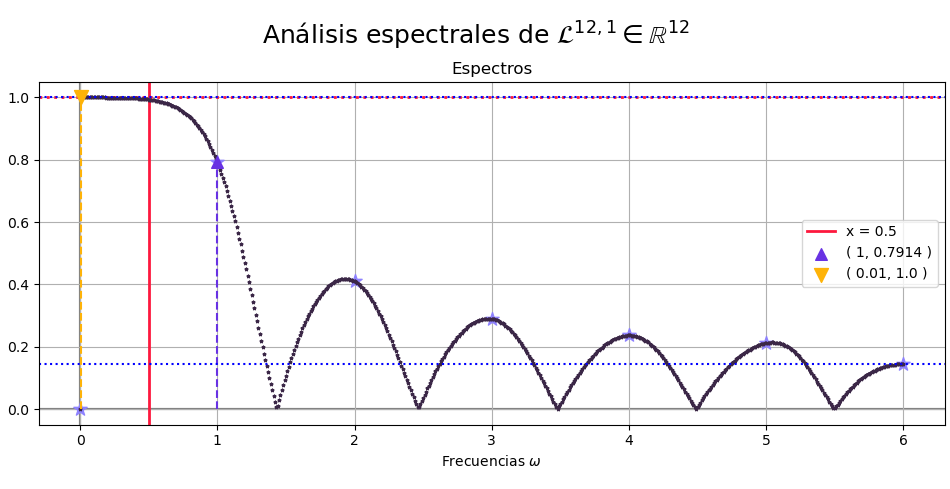
\includegraphics[scale = 0.5]{lim_1} 
\end{figure}	

\begin{figure}[H]
	\sidecaption{
	Observe que el espectro de $\cali{L}^{12,8}$ es, por el 
	contrario, continuo por $0$ pero discontinuo por $6$.
	\label{fig: lim 2}
	}
	\centering
	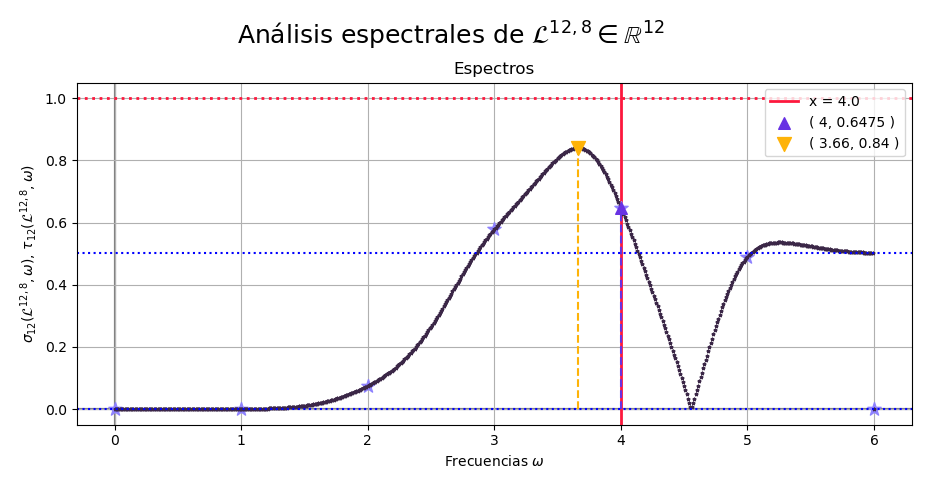
\includegraphics[scale = 0.5]{lim_2} 
\end{figure}

\begin{figure}[H]
	\sidecaption{
	El espectro de $\cali{L}^{12,9}$ es
	continuo por ambos extremos $0$ y $6$.
	\label{fig: lim 2}
	}
	\centering
	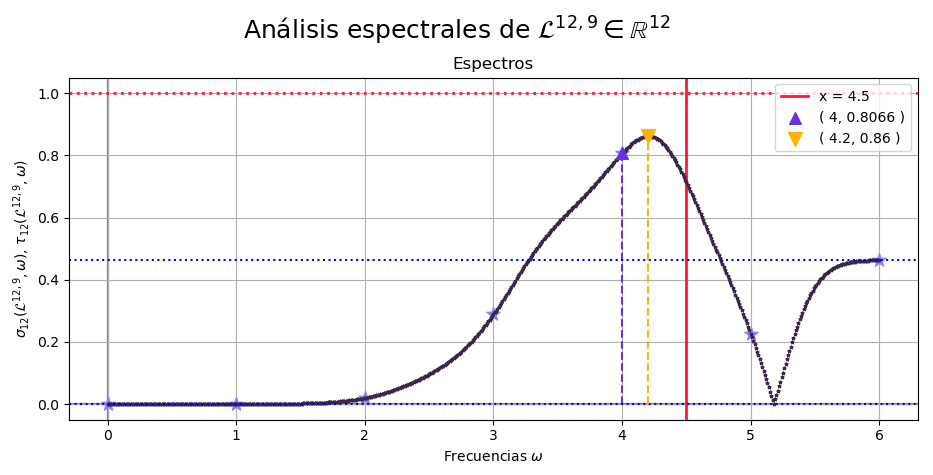
\includegraphics[scale = 0.5]{lim_3} 
\end{figure}

\begin{figure}[H]
	\sidecaption{
	El espectro de la señal
	$x = (1, 2, -3, -6) \in \IR^{4}$
	es discontinuo por ambos extremos
	$0$ y $2$.
	\label{fig: lim 4}
	}
	\centering
	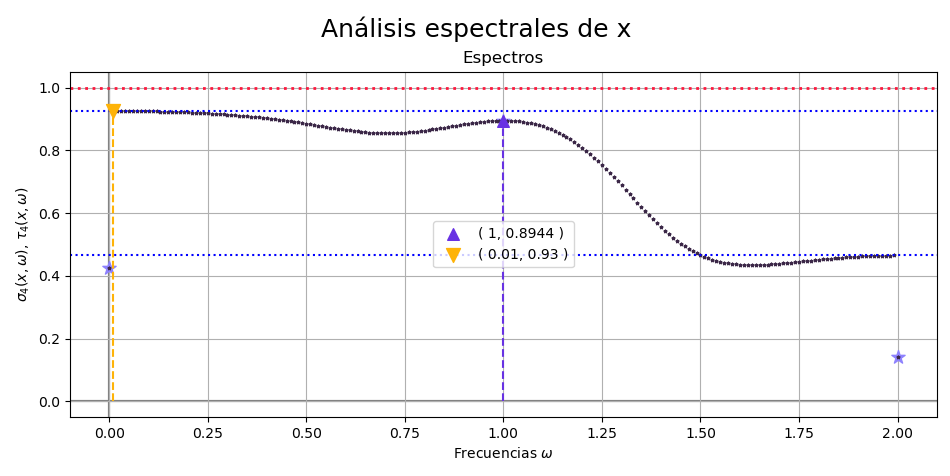
\includegraphics[scale = 0.5]{lim_4} 
\end{figure}


\section{Definición del espectro de una señal basado en espacios monofrecuenciales}

Estamos motivados a usar los coefcientes
$\sigma_{n}(x, \omega)$ de una señal $x$
(luego, a la función $\Sigma_{x}$ definida como en 
\eqref{eq: estudiando espectro}) para formular una definición
del espectro de una señal que indique qué tan cercana\sidenote{Midiéndose
tal cercanía con el coseno del ángulo que forma $x$ con espacios monofrecuenciales.}
es $x$ a pertenecer a un espacio monofrecuencia
$P_{n, \omega}$, luego, qué tan cercana es $x$ a tener
frecuencia pura $\omega$. Para nuestra definición, sería pertinente tomar
en cuenta que 

\begin{itemize}
\item $\Sigma_{x}$ es $n-$periódica, 
\item $\Sigma_{x}$ es simétrica respecto a la recta
vertical $\omega = n/2$, y
\item $\Sigma_{x}$ es continua en $]n/2[$ pero no necesariamente
en $0$ y $n/2$.
\end{itemize}
Estos primeros dos puntos se toman en cuenta al acotar
el dominio de frecuencias $\omega$, que en principio
era todo el rango $[0, \infty[$.

Nos gustaría que la función que sea el espectro de $x$
sea continua en todo su dominio
$[0, n/2]$. Según el último punto de la lista, tomando
directamente a la función $\Sigma_{x}$ (restringida a 
$[0,n/2]$), esto no puede asegurarse.
Como tenemos expresiones para los límites laterales, esto puede
remediarse fácilmente redefiniendo a 
$\Sigma_{x}$ en $0$ y $n/2$. Antes de hacer esto, 
establezcamos algunos resultados que nos ayudarán a expresar
a los límites de $\Sigma_{x}$ por $0$ y $n/2$
de una forma mucho más ilustrativa que la dada
en las fórmulas 
\eqref{eq: limite del espectro a cero}
y
\eqref{eq: limite del espectro a n medios}.

Para ello necesitamos antes el siguiente
\begin{lema}
Sean $n \neq 2$, $x \in \IR^{n}$.
Si
\begin{equation}
\label{ec: funcionales coordenadas}
c_{i}(x) := \langle x, \cali{L}^{m,i} \rangle,
\hspace{0.2cm} i = 0,1
\end{equation}
son los dos coeficientes primeros coeficientes
de $x$ respecto a la BLD $\cali{L}^{n,k}$,
entonces 
\begin{equation}
\label{ec: momento cero y coef 0}
M_{0}(x) = \sqrt{n} c_{0}(x)
\end{equation}
y
 \begin{equation}
\label{ec: momento cero y coef 1}
M_{1}(x) = \frac{c_{1}(x)}{\ell_{1}} + 
\frac{\sqrt{n}(n-1)}{2}c_{0}(x),
\end{equation}
donde
\begin{equation}
\label{ec: l1}
\ell_{1}:= \sqrt{\frac{
12
}{(n-1)n(n+1)}}.
\end{equation}
\end{lema}
\noindent
\textbf{Demostración.}
En efecto, según la ecuación
\eqref{eq: Ln, 0, m}, 
\[
c_{0}(x)= 
\langle x, \cali{L}^{n,0} \rangle
= \frac{1}{\sqrt{n}} \suma{m=0}{n-1}{x_{m}}
= \frac{1}{\sqrt{n}} M_{0}(x),
\]
luego, 
$M_{0}(x) = \sqrt{n} c_{0}$.
Además, según \eqref{eq: Ln, 1, m},
\[
c_{1}(x)= 
\langle x, \cali{L}^{m,1} \rangle
= \ell_{1} \suma{m=0}{n-1}{x_{m} \left(
m-  \frac{n-1}{2}
\right)}
= \ell_{1} \left(
M_{1}(x)-\frac{n-1}{2}M_{0}(x)
\right);
\]
despejando a $M_{1}(x)$ y usando la relación dada
de $M_{0}(x)$ obtenemos 
\eqref{ec: momento cero y coef 1}.
\QEDB
\vspace{0.2cm}

En la siguiente proposición establecemos
una interesante relación entre el espectro de una señal $x$
con sus primeros dos coeficientes respecto a la base
de Legendre discreta $\cali{L}^{n}$.
\begin{prop}
\label{prop: relacion limite cero con legendre}
Sean $n \geq 2$, $x \in \IR^{n}$,
$\Sigma_{x}$ el espectro de $x$.
Si $W_{n,1}$ es como en 
\eqref{espacios Wi}, el espacio
de los polinomios discretos de grado 
a lo más $1$ y dimensión $n$, entonces
\begin{equation}
\label{eq: limite por cero como angulo}
\limite{\omega \rightarrow 0^{+}}{
\Sigma_{x}(\omega)} = cos(\measuredangle(x, W_{n,1}))
\end{equation}
y
\begin{equation}
\label{eq: limite por cero como angulo}
\limite{\omega \rightarrow \frac{n}{2}^{-}}{
\Sigma_{x}(\omega)} = cos(\measuredangle(A_{n}(x), W_{n,1})).
\end{equation}
\end{prop}
\noindent
\textbf{Demostración.}
Según la proposición 
\ref{prop: proyecciones a espacios Wn,k}, 
\begin{equation}
\label{eq0: 25May23} 
||\Pi_{W_{n,1}}(x)|| = \sqrt{c_{0}(x)^{2} + c_{1}(x)^{2}},
\end{equation}
donde los $c_{i}$ son funcionales coordenada respecto
a la BON $\cali{L}^{n}$ como se definieron en 
\ref{ec: funcionales coordenadas}.

Sustituyendo las expresiones 
\eqref{ec: momento cero y coef 0} y
\eqref{ec: momento cero y coef 1} en la expresión 
\eqref{eq: limite del espectro a cero} del límite para 
$\limite{\omega \rightarrow 0^{+}}{\Sigma_{x}(\omega)}$,
tenemos que
\begin{align*}
\limite{\omega \rightarrow 0^{+}}{\Sigma_{x}(\omega)^{2}}
= & 
\left(
\frac{
2M_{0}(x)^{2}(2n-1)(n-1) + 12M_{1}(x)^{2} - 12M_{0}(x)M_{1}(x)(n-1)
}{
||x||^{2} (n-1)(n+1)n}
\right)^{1/2} \\
= & \frac{1}{||x||^{2}
(n-1)(n+1)n
} 
\left(
2nc_{0}(x)^{2}(n-1)(2n-1) + \right. \\
& \left.
12
\left(
\frac{c_{1}(x)}{\ell_{1}} + 
\frac{\sqrt{n}(n-1)}{2}c_{0}(x)
\right)^{2}-12
\sqrt{n} c_{0}(x) \sqrt{\frac{12}{
(n-1)n(n+1)
}} 
\right) \\
= & \frac{1}{||x||^{2}
(n-1)(n+1)n}
\left(
[2n(n-1)(2n-1) + \right. \\
& \left.
3n(n-1)^{2}-6(n-1)^{2}n]c_{0}(x)^{2}
+ \frac{12}{\ell^{2}_{1}}c_{1}(x)^{2}
\right) \\
= & \frac{c_{0}(x)^{2} + c_{1}(x)^{2}}{||x||^{2}}.
\end{align*}

\noindent
Usando \eqref{eq0: 25May23} podemos concluir
que
\[
\limite{\omega \rightarrow 0^{+}}{\Sigma_{x}(\omega)^{2}}
=  \frac{c_{0}(x)^{2} + c_{1}(x)^{2}}{||x||^{2}}
=  \frac{||\Pi_{W_{n,1}}(x)||}{||x||^{2}},
\]
siendo esta última expresión, según la proposición
\ref{prop: algunos hechos sobre el angulo entre un vector y un subespacio}, 
el coseno del ángulo que $x$ forma con $W_{n,1}$.  

Por último, usando
\eqref{eq: limite del espectro a n medios}
y lo ya demostrado se tiene que
$$\limite{\omega \rightarrow (n/2)^{-}}{\Sigma_{x}(\omega)}
= \limite{\omega \rightarrow 0^{+}}{\Sigma_{A_{n}(x)}(\omega)}
= \measuredangle(A_{n}(x), W_{n,1}).$$
\QEDB
\vspace{0.2cm}

\TODO{Aquí la explicación (+). Recuerda decir lo que en este
contexto significa la frecuencia cero, y cambiar más abajo
la observación sobre la extensión de este del espectro de fourier, pues
ya no va a a ser válida en los puntos extremos.}

Tenemos todo para definir el espectro de $x$
basado en espacios monofrecuenciales.

\begin{defi}
\label{def: espectro monofrecuenciales inicial}
\textbf{(Definición del espectro de una señal
basado en espacios monofrecuenciales)}
sean $n \geq 2$, $x \in \IR^{n}$. \\

Si $x \neq 0$, definimos a su \textbf{espectro basado
en espacios monofrecuenciales} como la función 
$\Sigma_{x}: [0, n/2] \longrightarrow [0,1]$
definida como
\begin{align*}
\Sigma_{x}(\omega)= \begin{cases}
cos(\measuredangle(x, P_{n, \omega})) & 
\hspace{0.2cm} \textit{ si } \omega \in ]0, n/2[, \\
cos(\measuredangle(x, W_{n,1})) & \hspace{0.2cm} \textit{ si } \omega = 0, \\
cos(\measuredangle(x, \tilde{W}_{n,1})) & \hspace{0.2cm} \textit{ si } \omega = n/2.
\end{cases}
\end{align*}

Si $x = 0$, definimos su espectro como la 
función constante cero.
\end{defi}


\begin{figure}[H]
	\sidecaption{
	Por definición, $\Sigma_{x}$ -el espectro de una señal 
	$x \in \IR^{n}$-es una función definida en $[0,n/2]$ y continua
	en su dominio. Preferimos no definir al espectro
	en $0$ y $n/2$ como el coseno del ángulo que forma $x$ con los 
	correspondientes espacios monofrecuenciales
	$P_{n,0}$ y $P_{n, \omega}$, pues esto daría lugar a una función
	que no siempre es continua en su dominio.
	\label{fig:angulos espectros}
	}
	\centering
	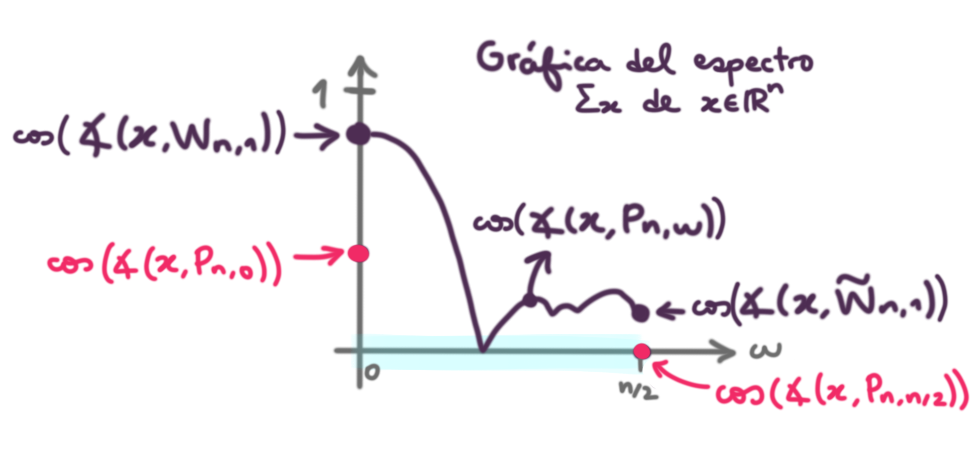
\includegraphics[scale = 1.5]{esp_ang} 
\end{figure}	

\begin{comment}
Esta última proposición es importante, pues relaciona
el espectro de una señal 
con sus primeros dos coeficientes respecto a la base
de Legendre discreta $\cali{L}^{n}$. \\
Note que este es un resultado razonable, pues, por
definición del espectro $\Sigma_{x}$, si $\omega \geq 0$,
$\Sigma_{x}(\omega)$ es el coseno del ángulo que
$x$ forma con el espacio $P_{n, \omega} = 
span \left\{ cos \left(
2 \pi \omega\frac{m}{n}
\right)_{m=0}^{n-1},  
sen \left(
2 \pi \omega\frac{m}{n}
\right)_{m=0}^{n-1} \right\}$, y, conforme
$\omega$ tiende a cero por la derecha, 
las discretizaciones de coseno y seno que generan
el espacio $P_{n, \omega}$ tienden a ser las discretizaciones
de cosenos y senos de muy baja frecuencia, luego, intuitivamente
son las discretizaciones de las rectas tangentes de un coseno
y un seno en $t =0$, que son las rectas $y=1$
y $y =x$. Observe que discretizaciones de estas dos rectas
conforman una base para el espacio $W_{n,1}$.
\end{comment}

\begin{prop}
\label{prop: formula explicita espectro}
Sean $n \neq 2$, $x \in \IR^{n}$ no cero.
Sea $\Sigma_{x}$ el espectro de $x$ como se definió en 
\ref{def: espectro monofrecuenciales inicial}.
Si $\omega \in ]0, n/2[$, entonces

\[
\Sigma_{x}(\omega) = 
\sigma_{n}(x, \omega) =
	\left(		  
		  \frac{\langle x, c_{n, \omega } \rangle^{2} +  \langle x, s_{n, \omega } \rangle^{2}	
	       -2  \langle x, c_{n, \omega } \rangle \langle x, s_{n, \omega } \rangle \langle c_{n, \omega }, s_{n, \omega } \rangle}{ || x ||^{2} \cdot
	       (1- \langle c_{n, \omega }, s_{n, \omega } \rangle^{2})}	  
\right) ^{1/2},
\]
donde los vectores $c_{n, \omega}$ y $s_{n, \omega}$
son como en \eqref{eq5: 19Marzo} y \eqref{eq6: 19Marzo}.
Además, 
\[
\Sigma_{x}(0) = 
\left(
\frac{
2M_{0}(x)^{2}(2n-1)(n-1) + 12M_{1}(x)^{2} - 12M_{0}(x)M_{1}(x)(n-1)
}{
||x||^{2} (n-1)(n+1)n}
\right)^{1/2}
\]
y
\[
\Sigma_{x}(n/2) = 
\left(
\frac{
2\tilde{M}_{0}(x)^{2}(2n-1)(n-1) + 12
\tilde{M}_{1}(x)^{2} - 12 \tilde{M}_{0}(x) \tilde{M}_{1}(x)(n-1)
}{
||x||^{2} (n-1)(n+1)n}
\right)^{1/2},
\]
donde los coeficientes $M_{i}(x)$ y $\tilde{M}_{i}(x)$
son como se definieron en 
\ref{def: momentos de x}. 
\end{prop}

Sólo para referenciar más adelante 
la continuidad del espectro de una 
señal y la forma en que se relacionan los valores
del espectro para pares de frecuencias $\omega$ y $n/2-\omega$,
plasmamos estos resultados 
-que son consecuencias directas de la forma en que hemos
definido el espectro $\Sigma_{x}$-
en la siguiente proposición.


\begin{prop}
\label{prop: continuidad espctro espacois monof.}
\textbf{(Propiedades importantes del espectro $\Sigma_{x}$ de una señal).}
Sean $n \geq 2$, $x \in \IR^{n}$.
Sea $\Sigma_{x}:[0, n/2] \rightarrow [0,1]$ el espectro 
de $x$ como se definió en 
\ref{def: espectro monofrecuenciales inicial}.
\begin{itemize}
	\item $\Sigma_{x}$ es una función continua.
	\item Para toda $\omega \in [0, n/4]$,
	\[
	\Sigma_{x}(n/2-\omega) = \Sigma_{A_{n}(x)}(\omega).
	\]
\end{itemize}
\end{prop}
\noindent
\textbf{Demostración.}
La continuidad de $\Sigma_{x}$ en el interior de
$[0, n/2]$ se estableció en
\ref{prop: cont interior espectro}, y la continuidad
en los puntos extremos $0$ y $n/2$
se sigue del
teorema \ref{teo: limite del espectro por cero},
la proposición
\ref{prop: relacion limite cero con legendre}
y la definición \ref{def: espectro monofrecuenciales inicial}
del espectro. \\

La veracidad del segundo punto para toda
$\omega \in ]0, n/4[$ se sigue directamente de 
la proposición 
\ref{prop: operaodr de alternancia y sigmas}. Por último,
haciendo $\omega = 0$ se tiene también la igualdad, pues

\begin{align*}
\Sigma_{x}(n/2) = &
\limite{\omega \rightarrow (n/2)^{-}}{\Sigma_{x}(n/2)} \\
= & \measuredangle(A_{n}(x)m W_{n,1}) \\
= & \limite{\omega \rightarrow 0^{+}}{ \Sigma_{A_{n}(x)}(\omega)} \\
= & \Sigma_{A_{n}(x)}(0),
\end{align*}
donde la primera y última igualdad son ciertas
por ser continuo el espectro $\Sigma_{x}$.
\QEDB
\vspace{0.2cm}

\begin{figure}[H]
	\sidecaption{
	Según la proposición 
	\ref{prop: continuidad espctro espacois monof.}, 
	si se quieren calcular los valores del espectro
	$\Sigma_{\cali{L}^{28,5}}$-
	cuyo dominio es $[0, 14]$- 
	en frecuencias $\omega \in [7, 14]$, estos pueden hallarse
	usando los valores del espectro del vector
	alternado $A_{28}(\cali{L}^{28,5})$ en el rango 
	de frecuencias $[0, 7]$. 
	\label{fig: espectro alternado}
	}
	\centering
	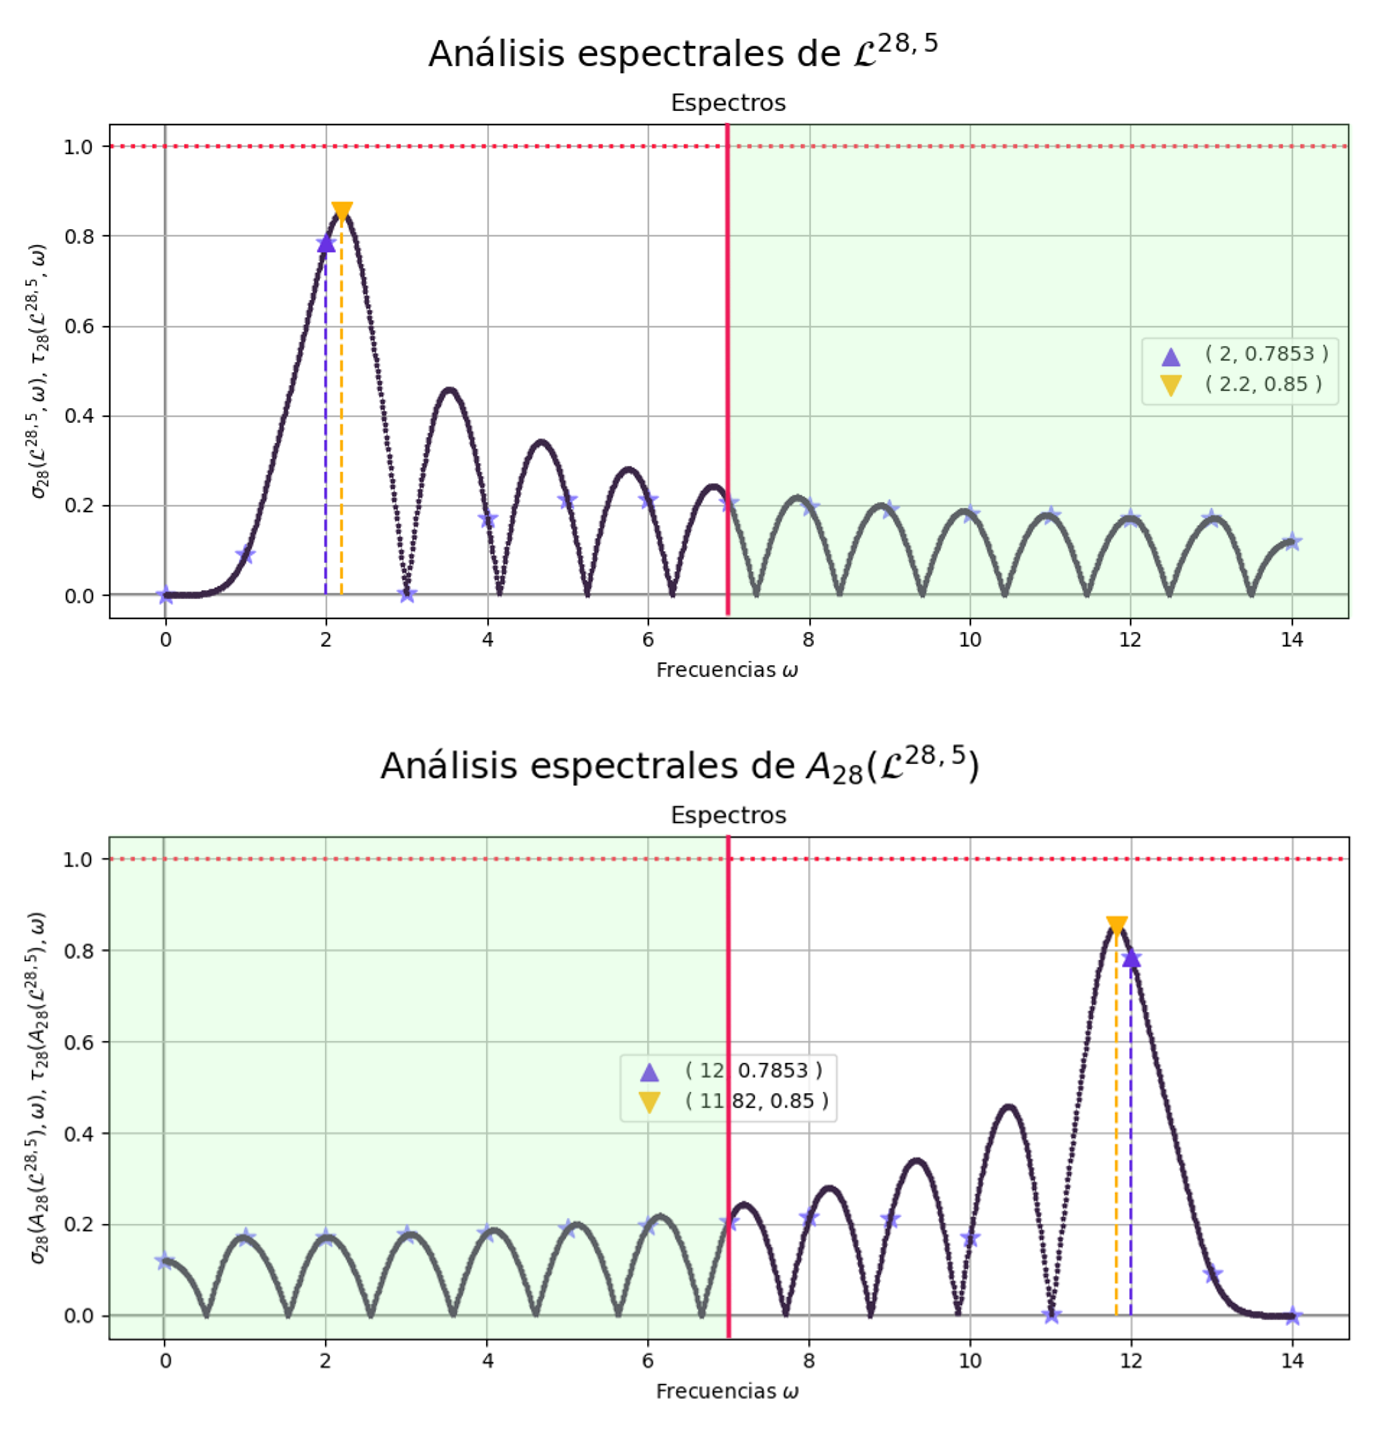
\includegraphics[scale = 1]{espectro_alternado} 
\end{figure}	
